% Compile with: tectonic reports/uav_oda_insight_slides.tex
\documentclass[10pt,aspectratio=169]{beamer}

\usepackage{fontspec}
\IfFileExists{/System/Library/Fonts/Supplemental/Arial.ttf}{
  \setmainfont[
    Path=/System/Library/Fonts/Supplemental/,
    UprightFont={Arial.ttf},
    BoldFont={Arial Bold.ttf},
    ItalicFont={Arial Italic.ttf},
    BoldItalicFont={Arial Bold Italic.ttf}
  ]{Arial}
  \setsansfont[
    Path=/System/Library/Fonts/Supplemental/,
    UprightFont={Arial.ttf},
    BoldFont={Arial Bold.ttf},
    ItalicFont={Arial Italic.ttf},
    BoldItalicFont={Arial Bold Italic.ttf}
  ]{Arial}
}{
  \IfFontExistsTF{Arial}{\setsansfont{Arial}\setmainfont{Arial}}{\setsansfont{TeX Gyre Heros}\setmainfont{TeX Gyre Heros}}
}
\usepackage{booktabs}
\usepackage{tabularx}
\usepackage{array}
\usepackage{graphicx}
\usepackage{adjustbox}
\usepackage{xcolor}
\usepackage{amsmath}
\usepackage{tikz}
\usetikzlibrary{positioning}

\graphicspath{{../outputs/figures/}{outputs/figures/}}

\definecolor{odaNavy}{HTML}{14213D}
\definecolor{odaBlue}{HTML}{2563EB}
\definecolor{odaCyan}{HTML}{0891B2}
\definecolor{odaGreen}{HTML}{15803D}
\definecolor{odaRed}{HTML}{B91C1C}
\definecolor{odaAmber}{HTML}{B45309}
\definecolor{odaGray}{HTML}{475569}
\definecolor{odaMuted}{HTML}{64748B}
\definecolor{odaLine}{HTML}{D8E1EF}
\definecolor{odaLight}{HTML}{F8FAFC}
\definecolor{odaPanel}{HTML}{EEF6FF}
\definecolor{odaInk}{HTML}{0F172A}

\usetheme{default}
\usefonttheme{professionalfonts}
\setbeamersize{text margin left=0.68cm,text margin right=0.68cm}
\setbeamertemplate{navigation symbols}{}
\setbeamertemplate{background canvas}{\color{odaLight}\vrule width\paperwidth height\paperheight}
\setbeamertemplate{footline}{
  \leavevmode%
  \hbox{%
    \begin{beamercolorbox}[wd=.78\paperwidth,ht=2.6ex,dp=1.05ex,leftskip=.68cm]{footline}
      \color{odaMuted}\scriptsize\insertshorttitle
    \end{beamercolorbox}%
    \begin{beamercolorbox}[wd=.22\paperwidth,ht=2.6ex,dp=1.05ex,rightskip=.68cm]{footline}
      \hfill\color{odaMuted}\scriptsize\insertframenumber/\inserttotalframenumber
    \end{beamercolorbox}%
  }%
  \begin{tikzpicture}[remember picture,overlay]
    \fill[odaLine] (current page.south west) rectangle ([yshift=1.3pt]current page.south east);
    \fill[odaBlue] (current page.south west) rectangle
      ([xshift=\paperwidth*\insertframenumber/\inserttotalframenumber,yshift=1.3pt]current page.south west);
  \end{tikzpicture}
}
\setbeamertemplate{frametitle}{
  \nointerlineskip
  \begin{beamercolorbox}[wd=\paperwidth,ht=1.07cm,dp=0cm,leftskip=.68cm,rightskip=.68cm]{frametitle}
    \vspace{0.27cm}
    {\color{odaNavy}\bfseries\large\insertframetitle\par}
  \end{beamercolorbox}
  \begin{tikzpicture}[remember picture,overlay]
    \fill[odaBlue] ([xshift=.68cm,yshift=-0.96cm]current page.north west) rectangle
      ([xshift=2.95cm,yshift=-1.00cm]current page.north west);
    \draw[odaLine,line width=.35pt] ([yshift=-1.07cm]current page.north west) --
      ([yshift=-1.07cm]current page.north east);
  \end{tikzpicture}
}
\setbeamercolor{normal text}{fg=odaInk,bg=odaLight}
\setbeamercolor{structure}{fg=odaBlue}
\setbeamercolor{frametitle}{fg=odaNavy,bg=white}
\setbeamercolor{title}{fg=odaNavy}
\setbeamercolor{subtitle}{fg=odaMuted}
\setbeamercolor{footline}{bg=white,fg=odaMuted}
\setbeamercolor{block title}{fg=odaNavy,bg=odaPanel}
\setbeamercolor{block body}{fg=odaInk,bg=odaPanel}
\setbeamerfont{title}{size=\Large,series=\bfseries}
\setbeamerfont{subtitle}{size=\normalsize}
\setbeamerfont{frametitle}{series=\bfseries}
\setbeamerfont{footline}{size=\scriptsize}
\setbeamertemplate{itemize item}{\color{odaBlue}\raisebox{0.15ex}{\scriptsize$\blacktriangleright$}}
\setbeamertemplate{itemize subitem}{\color{odaCyan}\scriptsize$\bullet$}
\setbeamertemplate{enumerate item}{\color{odaBlue}\bfseries\insertenumlabel.}

\newcommand{\insight}[1]{%
  \vspace{0.35em}
  \begin{beamercolorbox}[wd=\linewidth,sep=0.54em,rounded=true]{block body}
  
\begin{tikzpicture}[baseline=-0.6ex]
    \fill[odaBlue] (0,0) circle (0.08cm);
    \fill[odaCyan] (0.18,0) circle (0.08cm);
  \end{tikzpicture}\hspace{0.25em}%
  \color{odaNavy}\textbf{Insight.}\hspace{0.2em}\color{odaInk}#1
  \end{beamercolorbox}
}
\newcommand{\smallnote}[1]{{\scriptsize\color{odaMuted}#1}}
\newcommand{\code}[1]{\texttt{#1}}
\renewcommand{\arraystretch}{1.12}

\title{ODA-Bench}
\subtitle{A lightweight real-log benchmark for UAV obstacle avoidance}
\author[Nguyễn Thanh Lâm, Hoàng Công Phát]{Nguyễn Thanh Lâm \and Hoàng Công Phát}
\institute{Viettel High Tech}
\date{07/07/2026}

\begin{document}

\begin{frame}[plain]
  \begin{tikzpicture}[remember picture,overlay]
    \fill[white] (current page.south west) rectangle (current page.north east);
    \fill[odaNavy] (current page.south west) rectangle ([xshift=1.08cm]current page.north west);
    \fill[odaBlue] ([xshift=1.08cm]current page.south west) rectangle ([xshift=1.18cm]current page.north west);
    \fill[odaLight] ([xshift=1.18cm]current page.south west) rectangle (current page.north east);
    \fill[odaPanel] ([xshift=8.0cm,yshift=-.1cm]current page.north west) rectangle
      ([xshift=15.9cm,yshift=-8.9cm]current page.north west);
    \fill[odaCyan] ([xshift=8.0cm,yshift=-8.9cm]current page.north west) rectangle
      ([xshift=15.9cm,yshift=-8.98cm]current page.north west);
    \node[anchor=west,text width=6.45cm,align=left] at ([xshift=8.45cm,yshift=-2.1cm]current page.north west) {
      {\color{odaNavy}\bfseries\Large Real logs}\\[0.24cm]
      {\color{odaMuted}\normalsize ODA trajectories, sensor CSV, obstacle metadata.}
    };
    \node[anchor=west,text width=6.35cm,align=left] at ([xshift=8.45cm,yshift=-5.05cm]current page.north west) {
      {\color{odaBlue}\bfseries\large Offline benchmark}\\[0.18cm]
      {\color{odaInk}\normalsize Evaluate planners and lightweight learned policies before expensive field tests.}
    };
  \end{tikzpicture}
  \vspace{1.55cm}
  \hspace{1.25cm}
  \begin{minipage}{5.8cm}
  {\usebeamerfont{title}\color{odaNavy}\raggedright\hyphenpenalty=10000 ODA-Bench\\UAV Obstacle Avoidance\par}
  \vspace{0.38cm}
  {\usebeamerfont{subtitle}\color{odaMuted}Real-log offline evaluation\\for planning, risk and policy learning\par}
  \vspace{1.0cm}
  {\color{odaNavy}\bfseries Nguyễn Thanh Lâm\\Hoàng Công Phát\par}
  \vspace{0.15cm}
  {\color{odaMuted}\insertinstitute\par}
  \vfill
  {\scriptsize\color{odaMuted}Cập nhật: \insertdate}
\end{minipage}
\end{frame}

\begin{frame}{Abstract: ODA-Bench turns real logs into a benchmark}
\begin{columns}[T,onlytextwidth]
\column{0.52\linewidth}
\small
\textbf{\color{odaNavy}Problem}
\begin{itemize}
  \item UAV obstacle avoidance is risky to test directly because crashes are expensive.
  \item Simulation is useful, but sim-to-real gap makes offline real logs valuable.
  \item ODA provides real UAV logs, but not yet a standardized offline benchmark protocol.
\end{itemize}

\column{0.44\linewidth}
\small
\textbf{\color{odaNavy}Proposal}
\begin{itemize}
  \item Convert ODA logs into geometry, labels, tasks and baselines.
  \item Evaluate planners, BC policies and risk predictors offline.
  \item Validate candidate ranking with a lightweight simulator harness.
\end{itemize}
\end{columns}
\insight{Contribution nằm ở benchmark construction + evaluator + tasks + metrics + baselines + validation, không phải tạo raw ODA dataset mới.}
\end{frame}

\begin{frame}{The gap is between raw datasets and usable safety evaluation}
\begin{columns}[T,onlytextwidth]
\column{0.32\linewidth}
\begin{block}{Real logs}
\small
Trajectory and sensor evidence from real UAV flights, but no common task protocol.
\end{block}

\column{0.32\linewidth}
\begin{block}{Simulation}
\small
Closed-loop testing is controllable, but realism depends on sensor and dynamics fidelity.
\end{block}

\column{0.32\linewidth}
\begin{block}{Field tests}
\small
Most realistic, but slow, expensive and unsafe for early-stage candidates.
\end{block}
\end{columns}

\vspace{0.7em}
\begin{center}
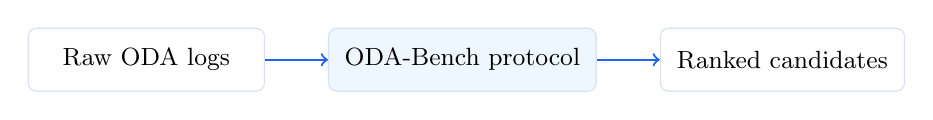
\begin{tikzpicture}[node distance=0.8cm]
  \node[draw=odaLine,fill=white,rounded corners=3pt,minimum width=3.0cm,minimum height=0.8cm] (raw) {\small Raw ODA logs};
  \node[draw=odaLine,fill=odaPanel,rounded corners=3pt,minimum width=3.4cm,minimum height=0.8cm,right=of raw] (bench) {\small ODA-Bench protocol};
  \node[draw=odaLine,fill=white,rounded corners=3pt,minimum width=3.1cm,minimum height=0.8cm,right=of bench] (rank) {\small Ranked candidates};
  \draw[->,thick,odaBlue] (raw) -- (bench);
  \draw[->,thick,odaBlue] (bench) -- (rank);
\end{tikzpicture}
\end{center}
\insight{ODA-Bench là lớp chuẩn hóa ở giữa: biến log thật thành metric có thể so sánh và dùng để lọc ứng viên trước simulator/field test.}
\end{frame}

\begin{frame}{Our contributions are benchmark components, not a new raw dataset}
\small
\begin{enumerate}
  \item We convert ODA real UAV logs into a standardized offline benchmark.
  \item We define collision, clearance, violation, latency-aware and learning metrics.
  \item We provide planner, imitation learning and risk prediction tracks with lightweight baselines.
  \item We implement a simulation validation harness for ranking candidates before field testing.
\end{enumerate}

\vspace{0.6em}
\begin{columns}[T,onlytextwidth]
\column{0.48\linewidth}
\begin{block}{Current evidence}
\small
300 ODA trial CSV subset, 14,700 expert samples, 4 baseline families, 3 main plots.
\end{block}
\column{0.48\linewidth}
\begin{block}{Scope boundary}
\small
No claim of field safety or PX4 closed-loop safety. PyBullet backend is implemented; execution is pending on a compatible machine.
\end{block}
\end{columns}
\end{frame}

\begin{frame}{Related work leaves a real-log benchmark gap}
\small
\begin{columns}[T,onlytextwidth]
\column{0.48\linewidth}
\textbf{\color{odaNavy}Existing directions}
\begin{itemize}
  \item UAV obstacle avoidance datasets capture real sensor/trajectory evidence.
  \item Simulation benchmarks test closed-loop controllers under controlled settings.
  \item Learning-based avoidance evaluates policies, often with synthetic or simulator-heavy data.
  \item Offline RL benchmarks define logged transitions and cost/reward protocols.
\end{itemize}

\column{0.48\linewidth}
\textbf{\color{odaNavy}What is missing}
\begin{itemize}
  \item A trial-level split and evaluator on real UAV logs.
  \item Shared safety labels for collision, violation and clearance.
  \item Comparable tracks for planners, BC and risk models.
  \item A lightweight bridge from offline ranking to simulator validation.
\end{itemize}
\end{columns}
\insight{Unlike prior workflows, ODA-Bench uses real UAV logs and supports both offline evaluation and lightweight offline policy training.}
\end{frame}

\begin{frame}{ODA-Bench construction: from CSV logs to benchmark cases}
\begin{columns}[T,onlytextwidth]
\column{0.47\linewidth}
\small
\textbf{\color{odaNavy}Raw input used}
\begin{itemize}
  \item 300 local ODA trials downloaded from Hugging Face.
  \item 300 \code{optitrack.csv}, 300 \code{imu.csv}, 300 \code{radar.csv}.
  \item Trial metadata gives obstacle position, light condition and video flags.
\end{itemize}

\vspace{0.2em}
\textbf{\color{odaNavy}Geometry proxy}
\[
\mathbf{p}_t=(x_t,z_t),\qquad \mathbf{o}_j=(x_j,z_j)
\]
\[
c_t=\min_j\|\mathbf{p}_t-\mathbf{o}_j\|_2-r_{\mathrm{obs}}
\]

\column{0.49\linewidth}
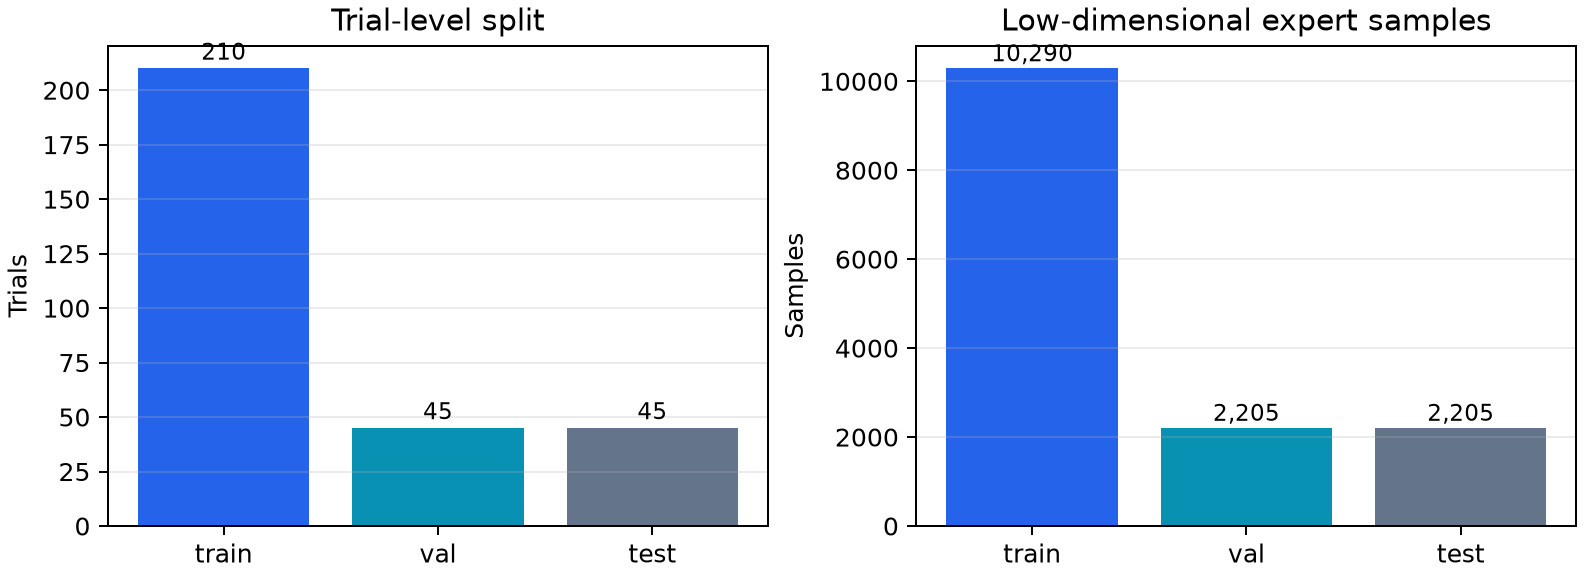
\includegraphics[width=\linewidth,height=0.52\textheight,keepaspectratio]{oda_bench_split_300.png}
\end{columns}
\smallnote{Split is by trial ID, not by random timestep, to reduce leakage across train/val/test.}
\end{frame}

\begin{frame}{Evaluation labels separate contact from near-miss risk}
\setlength{\abovedisplayskip}{2pt}
\setlength{\belowdisplayskip}{2pt}
\begin{columns}[T,onlytextwidth]
\column{0.50\linewidth}
\small
\textbf{\color{odaNavy}Clearance over a trajectory}
\[
c_{\min}=\min_t c_t
\]

\textbf{\color{odaNavy}Safety labels}
\[
\mathrm{collision}=\mathbb{1}[c_{\min}\le 0]
\]
\[
\mathrm{violation}=\mathbb{1}[0<c_{\min}<r_{\mathrm{safe}}]
\]

\column{0.46\linewidth}
\small
\textbf{\color{odaNavy}Constants}
\begin{adjustbox}{max width=\linewidth}
\begin{tabular}{lrl}
\toprule
Symbol & Value & Meaning \\
\midrule
\(r_{\mathrm{obs}}\) & 0.20 m & contact radius \\
\(r_{\mathrm{safe}}\) & 0.50 m & safety margin \\
\(r_{\mathrm{obs}}+r_{\mathrm{safe}}\) & 0.70 m & violation boundary \\
\bottomrule
\end{tabular}
\end{adjustbox}

\vspace{0.5em}
\textbf{\color{odaNavy}Latency proxy}
\[
d_{\mathrm{delay}}=\|\mathbf{v}\|T_{\mathrm{delay}}
\]
\[
T_{\mathrm{delay}}=T_{\mathrm{sensor}}+T_{\mathrm{map}}+T_{\mathrm{planner}}+T_{\mathrm{cmd}}
\]
\end{columns}
\insight{Collision is contact. Violation is a near-miss inside the safety ring, which is useful for ranking before actual crashes happen.}
\end{frame}

\begin{frame}{The benchmark defines four downstream tracks}
\small
\begin{adjustbox}{max width=\linewidth}
\begin{tabular}{p{2.7cm}p{3.2cm}p{3.1cm}p{4.2cm}}
\toprule
Track & Input & Output & Primary metrics \\
\midrule
Offline planner & start, goal, obstacles & path/trajectory & collision, violation, clearance, length, runtime \\
Filtered BC & expert trajectories & local waypoint action & action MSE, rollout safety, inference latency \\
Risk prediction & state/sensor features & future-risk score & PR-AUC, recall, false negative, calibration \\
Offline RL & logged transitions & learned policy & return, cost, collision, sim validation \\
\bottomrule
\end{tabular}
\end{adjustbox}

\vspace{0.8em}
\begin{columns}[T,onlytextwidth]
\column{0.48\linewidth}
\begin{block}{Main claim tracks}
\small
Planner, BC and risk are fully run on the 300-trial CSV subset.
\end{block}
\column{0.48\linewidth}
\begin{block}{Stretch track}
\small
Offline RL is kept as future work until TD3+BC/IQL/Decision Transformer baselines are validated.
\end{block}
\end{columns}
\end{frame}

\begin{frame}{Baselines are intentionally lightweight and reproducible}
\small
\begin{columns}[T,onlytextwidth]
\column{0.48\linewidth}
\textbf{\color{odaNavy}Main baselines}
\begin{itemize}
  \item Planner: RRT* and MPPI.
  \item Behavior cloning: Plain BC-MPPI and Filtered BC-MPPI.
  \item Risk: TTC/clearance threshold and Small MLP.
  \item Validation: ODA-like obstacle course, 20 seeds \(\times\) 4 speeds.
\end{itemize}

\column{0.48\linewidth}
\textbf{\color{odaNavy}Kept out of main story}
\begin{itemize}
  \item RRT, A*, straight-line and human trajectory: useful appendix references.
  \item Heavy offline RL: not a main claim until simulation results are stable.
  \item Real flight safety: explicitly out of scope.
\end{itemize}
\end{columns}
\insight{The benchmark is designed to run on MacBook-class hardware first, then validate finalists in a simulator.}
\end{frame}

\begin{frame}{RQ1: ODA-Bench separates unsafe baselines from safe planners}
\begin{columns}[T,onlytextwidth]
\column{0.64\linewidth}
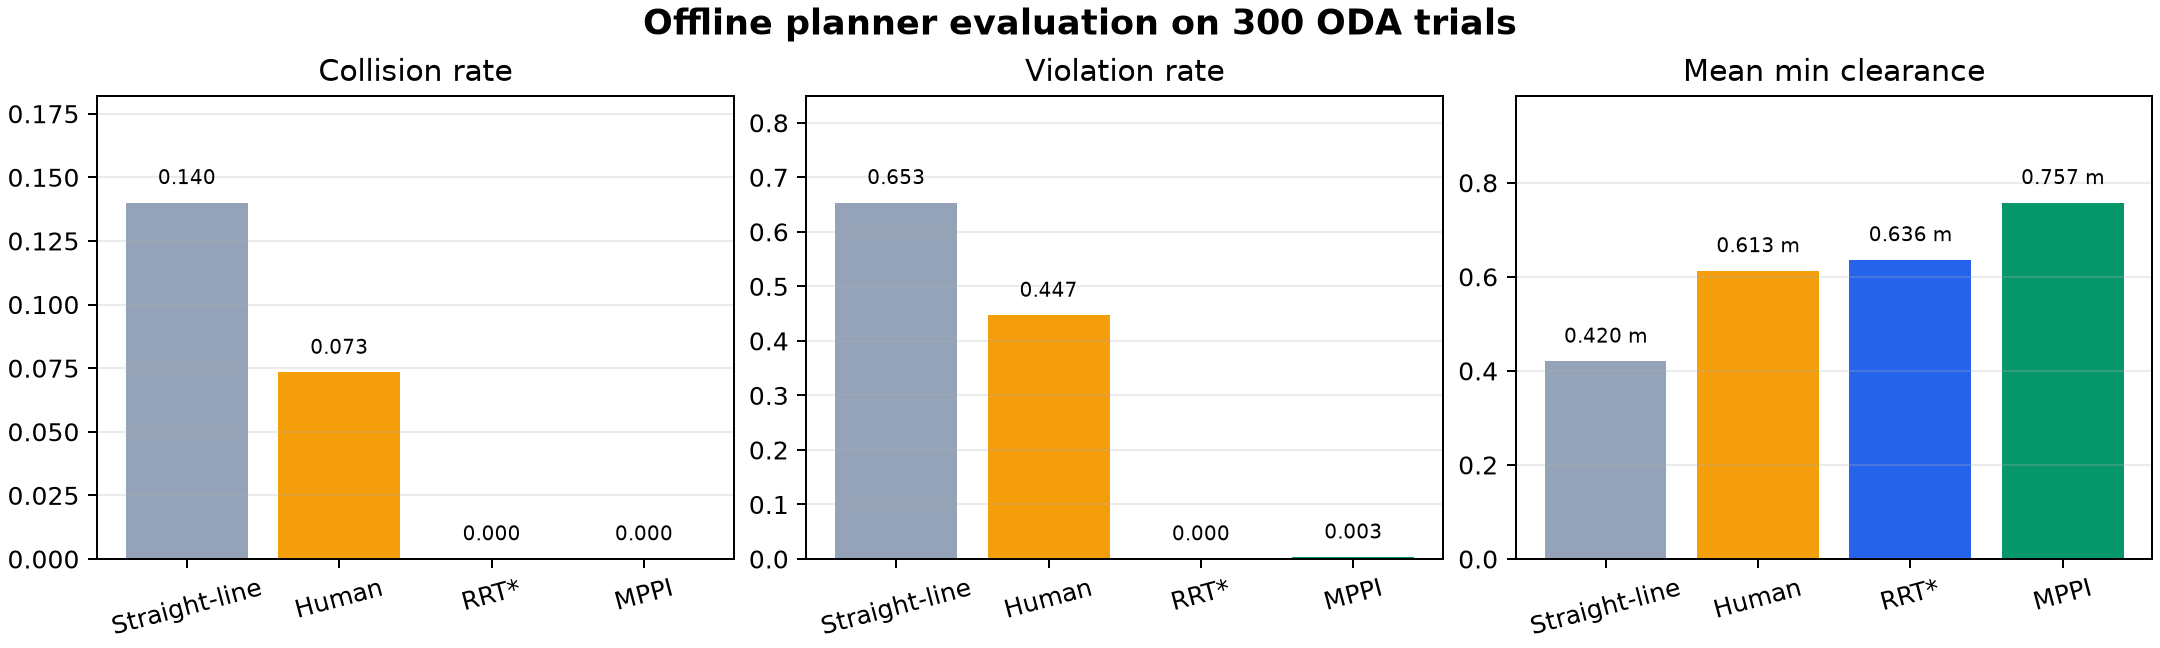
\includegraphics[width=\linewidth,height=0.63\textheight,keepaspectratio]{oda_planner_safety_300.png}

\column{0.32\linewidth}
\small
\textbf{\color{odaNavy}Main readout}
\begin{itemize}
  \item Straight-line has high collision and violation.
  \item RRT* reaches zero collision and zero violation on the 300-trial geometry benchmark.
  \item MPPI reaches zero collision and the highest clearance among main planners.
\end{itemize}
\end{columns}
\smallnote{Human/OptiTrack is a real flight trajectory reference, not an optimal planner. Main comparison should focus on RRT* vs MPPI.}
\end{frame}

\begin{frame}{Planner safety and compute trade off differently}
\begin{columns}[T,onlytextwidth]
\column{0.49\linewidth}
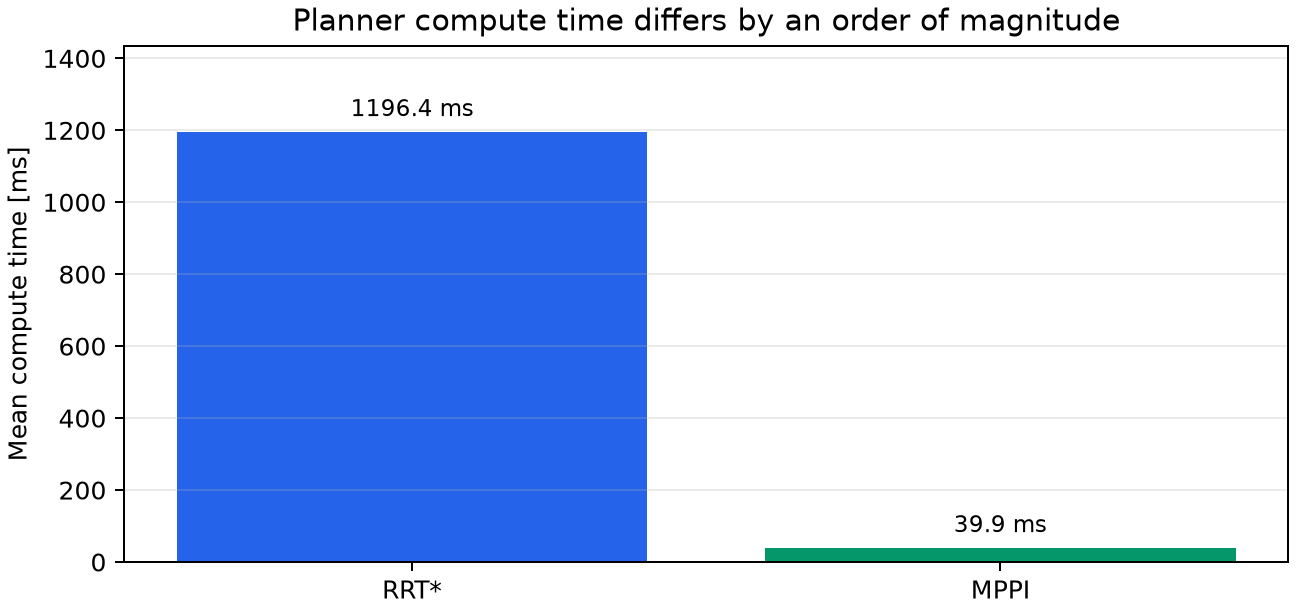
\includegraphics[width=\linewidth,height=0.50\textheight,keepaspectratio]{oda_planner_compute_rrtstar_mppi.png}
\column{0.47\linewidth}
\small
\textbf{\color{odaNavy}RRT* vs MPPI on 300 ODA trials}
\begin{itemize}
  \item RRT*: collision \(0.0000\), violation \(0.0000\), clearance \(0.6360\) m.
  \item MPPI: collision \(0.0000\), violation \(0.0033\), clearance \(0.7574\) m.
  \item Mean compute time: RRT* \(1196.4\) ms vs MPPI \(39.9\) ms.
\end{itemize}
\end{columns}
\insight{Offline safety alone is not enough for online UAV use. Compute and sensor delay determine whether a safe path arrives in time.}
\end{frame}

\begin{frame}{RQ2: filtering expert samples improves BC safety}
\begin{columns}[T,onlytextwidth]
\column{0.64\linewidth}
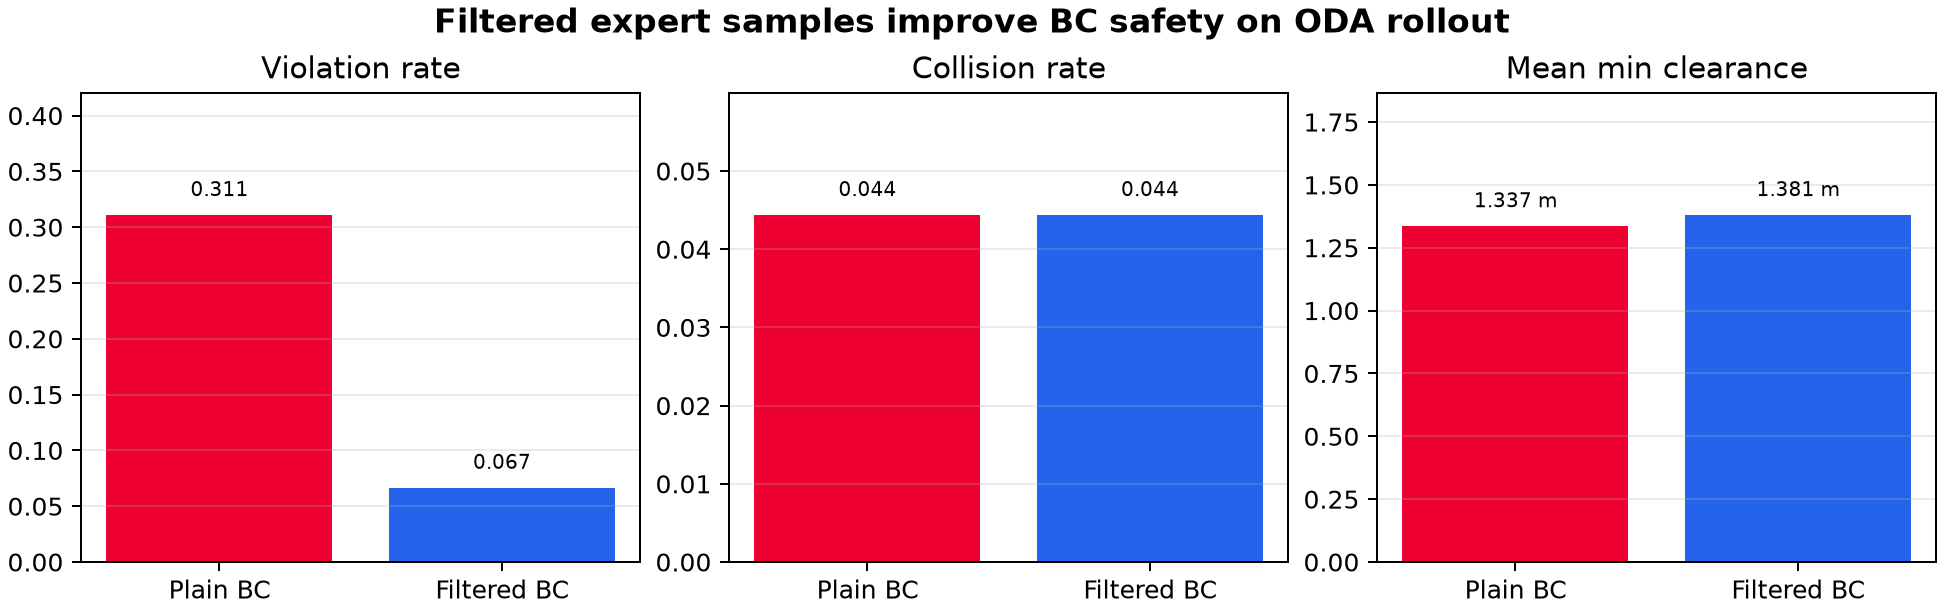
\includegraphics[width=\linewidth,height=0.62\textheight,keepaspectratio]{bc_filtered_vs_plain_300.png}

\column{0.32\linewidth}
\small
\textbf{\color{odaNavy}300-trial split}
\begin{itemize}
  \item Train: 210 trials, 10,290 samples.
  \item Val: 45 trials, 2,205 samples.
  \item Test: 45 trials, 2,205 samples.
\end{itemize}
\vspace{0.2em}
\textbf{\color{odaNavy}Result}
\begin{itemize}
  \item Violation drops from \(0.3111\) to \(0.0667\).
  \item Clearance increases from \(1.3365\) m to \(1.3809\) m.
\end{itemize}
\end{columns}
\smallnote{Collision rate is tied at 0.0444; filtered BC improves near-miss behavior more clearly than contact rate on this split.}
\end{frame}

\begin{frame}{RQ3: ODA risk labels support useful future-risk prediction}
\begin{columns}[T,onlytextwidth]
\column{0.62\linewidth}
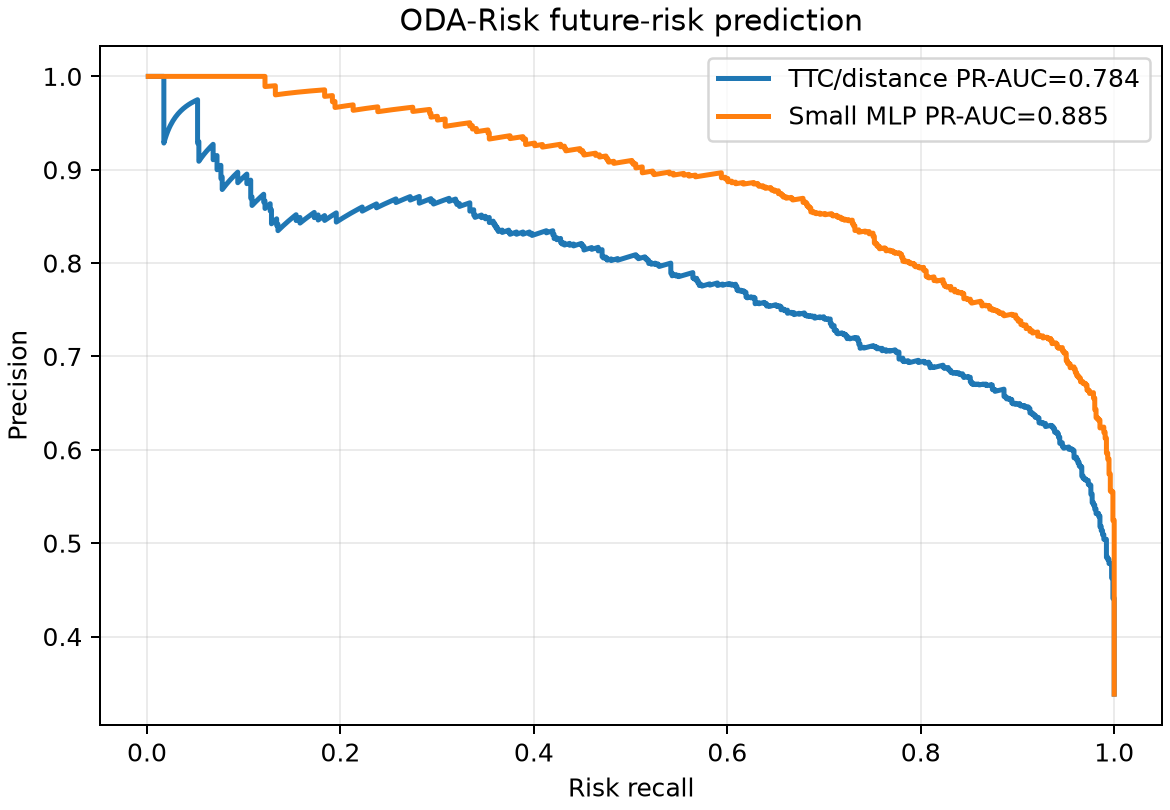
\includegraphics[width=\linewidth,height=0.56\textheight,keepaspectratio]{risk_predictor_pr_curve.png}

\column{0.34\linewidth}
\small
\textbf{\color{odaNavy}Test set}
\begin{itemize}
  \item 2,205 samples.
  \item Positive rate: 0.3383.
\end{itemize}
\vspace{0.2em}
\textbf{\color{odaNavy}Small MLP vs TTC}
\begin{itemize}
  \item PR-AUC: \(0.885\) vs \(0.784\).
  \item Risk recall: \(0.992\).
  \item False negative rate: \(0.008\).
\end{itemize}
\end{columns}
\insight{For rare safety events, PR-AUC, recall and false negatives are more meaningful than accuracy.}
\end{frame}

\begin{frame}{RQ4: validation harness ranks candidates before heavy simulation}
\begin{columns}[T,onlytextwidth]
\column{0.61\linewidth}
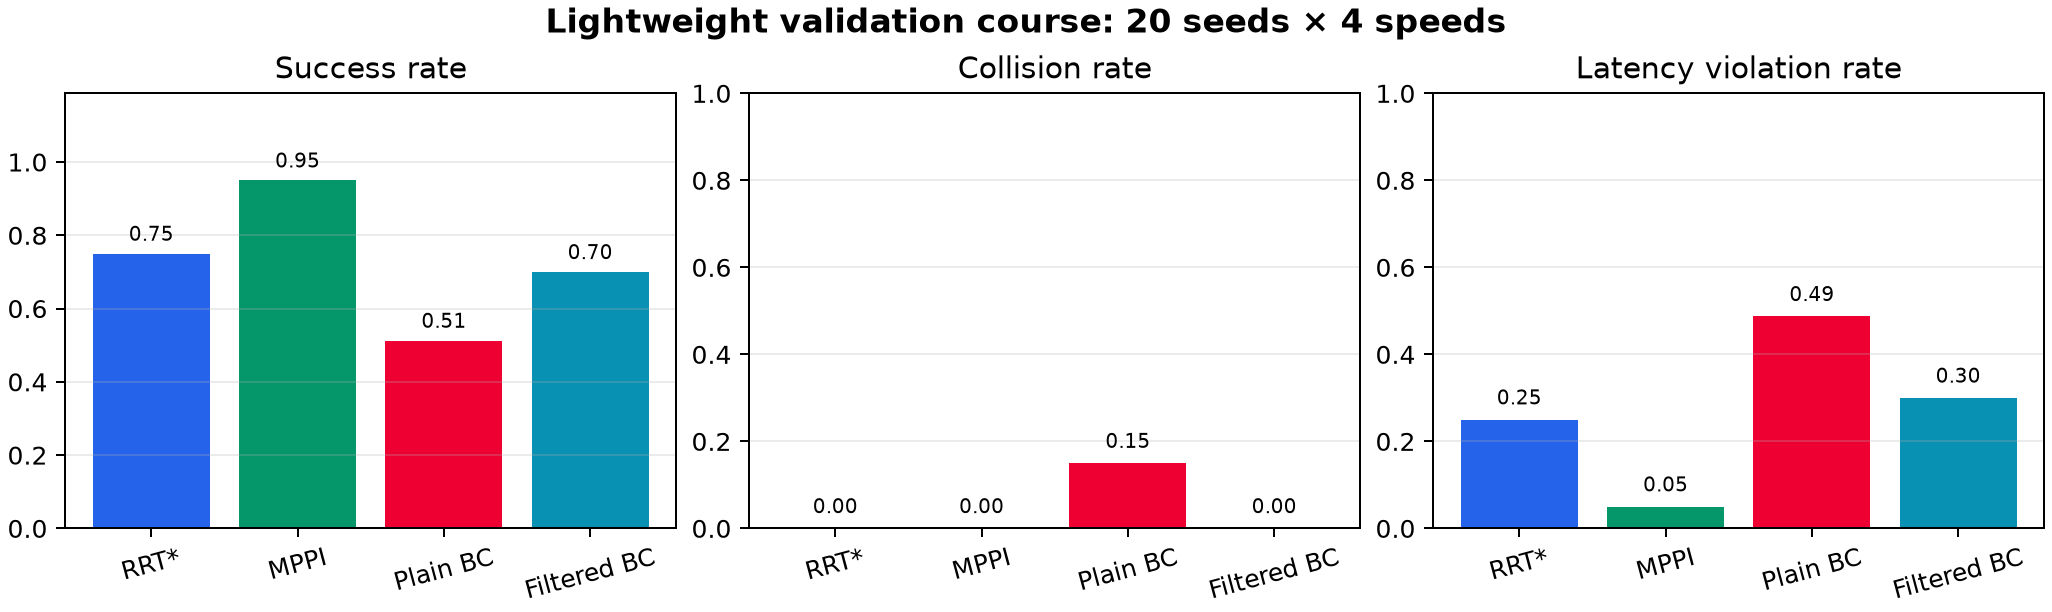
\includegraphics[width=\linewidth,height=0.60\textheight,keepaspectratio]{validation_course_summary.png}

\column{0.35\linewidth}
\small
\textbf{\color{odaNavy}Current run}
\begin{itemize}
  \item 20 seeds \(\times\) 4 speed levels.
  \item Backend: kinematic fallback.
  \item MPPI has highest success: \(0.95\).
  \item Plain BC shows worst collision: \(0.15\).
\end{itemize}
\end{columns}
\smallnote{The gym-pybullet-drones backend is implemented with CtrlAviary + DSLPIDControl, but PyBullet did not build on the current Apple Silicon environment. The GTX machine should run the true PyBullet validation.}
\end{frame}

\begin{frame}{RQ5: offline ranking currently agrees only partially with validation}
\begin{columns}[T,onlytextwidth]
\column{0.58\linewidth}
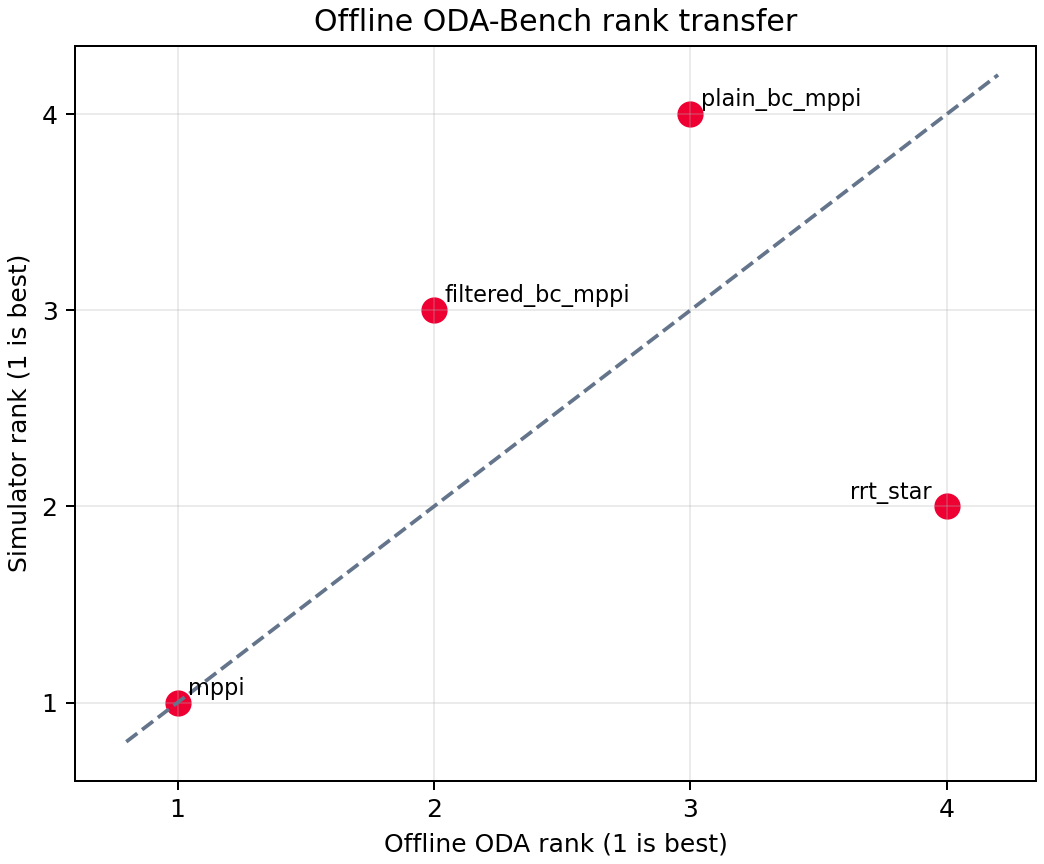
\includegraphics[width=\linewidth,height=0.56\textheight,keepaspectratio]{offline_vs_sim_rank_correlation.png}

\column{0.38\linewidth}
\small
\textbf{\color{odaNavy}Rank transfer}
\begin{itemize}
  \item Spearman \(\rho=0.4\) on current fallback validation.
  \item Offline rank 1 and validation rank 1 both select MPPI.
  \item BC methods diverge more, exposing failure cases that need simulator checks.
\end{itemize}
\end{columns}
\insight{ODA-Bench is useful as an early filter; PyBullet validation is still needed before stronger claims.}
\end{frame}

\begin{frame}{Discussion: what ODA-Bench can and cannot claim today}
\small
\begin{columns}[T,onlytextwidth]
\column{0.48\linewidth}
\textbf{\color{odaNavy}What the evidence supports}
\begin{itemize}
  \item ODA can be converted into repeatable offline safety labels.
  \item Planner, BC and risk tracks run on a 300-trial trial-level split.
  \item Filtered BC reduces violation.
  \item Small MLP risk predictor improves PR-AUC over TTC.
\end{itemize}

\column{0.48\linewidth}
\textbf{\color{odaNavy}What remains limited}
\begin{itemize}
  \item Offline geometry does not replace closed-loop dynamics.
  \item Kinematic fallback is not equivalent to PyBullet or real UAV flight.
  \item ODA scenes are limited by available obstacle metadata and sensor noise.
  \item Offline RL is a future track, not a main result yet.
\end{itemize}
\end{columns}
\end{frame}

\begin{frame}{Conclusion: ODA-Bench is a practical bridge before field testing}
\small
\begin{columns}[T,onlytextwidth]
\column{0.48\linewidth}
\textbf{\color{odaNavy}Core message}
\begin{itemize}
  \item We propose an evaluation protocol and benchmark suite built on top of ODA.
  \item It supports offline planner evaluation, lightweight policy training and risk prediction.
  \item It reduces dependence on simulation-heavy workflows for early candidate screening.
\end{itemize}

\column{0.48\linewidth}
\textbf{\color{odaNavy}Next step}
\begin{itemize}
  \item Run the implemented gym-pybullet-drones backend on the GTX 1050 Ti machine.
  \item Replace fallback validation with PyBullet ranks.
  \item Add TD3+BC/IQL only if the simulator validation is stable.
\end{itemize}
\end{columns}
\insight{The final paper claim should be benchmark + evaluator + tasks + baselines + lightweight validation, not field-ready UAV autonomy.}
\end{frame}

\end{document}
